%
% "Data Analysis in R", CS 50 seminar
% Author: Dustin Tran <dustinvtran.com>
%
% This requires compiling with xelatex because it uses a custom font; make sure
% you also have the fonts installed on your PC, as well as the packages listed
% here.

%##############################################################################
% Preamble
%##############################################################################
\documentclass[10pt,c]{beamer}
\usepackage{tikz}
\usepackage{fontspec, xunicode}
\usepackage{listings}
\usepackage{hyperref}

\setmainfont[Mapping=tex-text]{Helvetica Neue Thin}
\let\sfdefault\rmdefault
\setmonofont[Mapping=tex-text]{Courier New}

\setbeamertemplate{navigation symbols}{}
\setbeamertemplate{frametitle}{\vspace{3ex}\centerline{\insertframetitle}}
\setbeamertemplate{itemize items}[circle]

\definecolor{charcoal}{HTML}{222222}
\definecolor{snow}{HTML}{F9F9F9}
\setbeamercolor{structure}{fg=snow}
\setbeamercolor{background canvas}{bg=charcoal}
\setbeamercolor{section in head/foot}{bg=white}
\setbeamercolor{normal text}{fg=snow}
\definecolor{github-blue}{HTML}{4183C4}
\hypersetup{colorlinks=true,urlcolor=github-blue}

\definecolor{fgcolor}{rgb}{0.345, 0.345, 0.345}
\definecolor{hlnum}{rgb}{0.686,0.059,0.569}
\definecolor{hlstr}{rgb}{0.192,0.494,0.8}
\definecolor{hlcom}{rgb}{0.678,0.584,0.686}
\definecolor{hlopt}{rgb}{0,0,0}
\definecolor{hlstd}{rgb}{0.345,0.345,0.345}
\definecolor{hlkwa}{rgb}{0.161,0.373,0.58}
\definecolor{hlkwb}{rgb}{0.69,0.353,0.396}
\definecolor{hlkwc}{rgb}{0.333,0.667,0.333}
\definecolor{hlkwd}{rgb}{0.737,0.353,0.396}
\definecolor{shadecolor}{rgb}{0.969, 0.969, 0.969}

\definecolor{monokai-purple}{HTML}{AE81FF}
\definecolor{monokai-red}{HTML}{F92672}
\definecolor{monokai-gray}{HTML}{75715E}
\definecolor{monokai-green}{HTML}{A6E22E}
\lstdefinelanguage{Renhanced}{
  comment=[l][\color{monokai-gray}]{\#},
  alsoletter={>,<,-,+,=,*,!,:},
  columns=fullflexible,
  keepspaces=true,
  keywords=[2]{for,in,<-},
  keywords=[3]{NA,TRUE,FALSE},
  keywords=[4]{-,+,=,*,>,<,!,!=,>=,<=},
  %keywords=[5]{[,]},
  keywords=[5]{:},
  keywordstyle=\color{monokai-red},
  keywordstyle=[2]{\color{monokai-red}},
  keywordstyle=[3]{\color{monokai-purple}},
  keywordstyle=[4]{\color{monokai-green}},
  keywordstyle=[5]{\color{monokai-gray}},
  literate=%
          *{0}{{\color{monokai-purple}{0}}}{1}%
           {1}{{\color{monokai-purple}{1}}}{1}%
           {2}{{\color{monokai-purple}{2}}}{1}%
           {3}{{\color{monokai-purple}{3}}}{1}%
           {4}{{\color{monokai-purple}{4}}}{1}%
           {5}{{\color{monokai-purple}{5}}}{1}%
           {6}{{\color{monokai-purple}{6}}}{1}%
           {7}{{\color{monokai-purple}{7}}}{1}%
           {8}{{\color{monokai-purple}{8}}}{1}%
           {9}{{\color{monokai-purple}{9}}}{1}%
           {.0}{{\color{monokai-purple}{.0}}}{2}%
           {.1}{{\color{monokai-purple}{.1}}}{2}%
           {.2}{{\color{monokai-purple}{.2}}}{2}%
           {.3}{{\color{monokai-purple}{.3}}}{2}%
           {.4}{{\color{monokai-purple}{.4}}}{2}%
           {.5}{{\color{monokai-purple}{.5}}}{2}%
           {.6}{{\color{monokai-purple}{.6}}}{2}%
           {.7}{{\color{monokai-purple}{.7}}}{2}%
           {.8}{{\color{monokai-purple}{.8}}}{2}%
           {.9}{{\color{monokai-purple}{.9}}}{2}%
           {0L}{{\color{monokai-purple}{0L}}}{2}%
           {1L}{{\color{monokai-purple}{1L}}}{2}%
           {2L}{{\color{monokai-purple}{2L}}}{2}%
           {3L}{{\color{monokai-purple}{3L}}}{2}%
           {4L}{{\color{monokai-purple}{4L}}}{2}%
           {5L}{{\color{monokai-purple}{5L}}}{2}%
           {6L}{{\color{monokai-purple}{6L}}}{2}%
           {7L}{{\color{monokai-purple}{7L}}}{2}%
           {8L}{{\color{monokai-purple}{8L}}}{2}%
           {9L}{{\color{monokai-purple}{9L}}}{2}%
           {[}{{\color{monokai-gray}{[}}}{1}%
           {]}{{\color{monokai-gray}{]}}}{1}%
           {\{}{{\color{monokai-gray}{\{}}}{2}%
           {\}}{{\color{monokai-gray}{\}}}}{2}%
           {(}{{\color{monokai-gray}{(}}}{1}%
           {)}{{\color{monokai-gray}{)}}}{1}%
           {^}{{\color{monokai-green}{\^{}}}}{1}%
           {\%\%}{{\color{monokai-green}{\%\%}}}{2}%
           {\%/\%}{{\color{monokai-green}{\%/\%}}}{3}%
           {\%*\%}{{\color{monokai-green}{\%*\%}}}{3}%
           {TRUE\,}{{\color{monokai-purple}{TRUE}},}{5}%
           {FALSE\,}{{\color{monokai-purple}{FALSE}},}{6}%
           ,
           %string yellow
           %\" as gray
}
\lstset{
  language=Renhanced,
  basicstyle=\Large\ttfamily,
}
\newcommand{\tinybullet}{$\vcenter{\hbox{\tiny$\bullet$}}$}
\makeatletter
\DeclareRobustCommand{\em}{%
  \color{monokai-red}
  }
\makeatother

\newenvironment{changemargin}[1]{
  \begin{list}{}{
    \setlength{\topsep}{0pt}
    \setlength{\leftmargin}{#1}
    \setlength{\rightmargin}{#1}
    \setlength{\listparindent}{\parindent}
    \setlength{\itemindent}{\parindent}
    \setlength{\parsep}{\parskip}
  }
  \item[]}{\end{list}}

\title{}
\begin{document}
%##############################################################################
% Frames
%##############################################################################
% Default frame dimensions are 12.8cm x 9.6cm
\begingroup
\setbeamercolor{background canvas}{bg=custom-red}
\begin{frame}[plain,t]
\vspace{4cm}
\hspace{0.5cm}
{\huge Data Analysis in R}\\[2ex]
\hspace{0.5cm}
@dustinvtran\\
\hspace{0.5cm}
Engineering and Applied Sciences @\\
\hspace{0.5cm}
Harvard University\\
\end{frame}
\endgroup
\begin{frame}[plain]
\vspace{1.5cm}
\begin{center}
\Large\texttt{1. introduction}
\end{center}
\end{frame}
\begin{frame}
\frametitle{What is R?}
\begin{itemize}[<+->]
\item R is a language \emph{developed for statistical computing and
visualization}
\item It is \emph{free} and \emph{open source}
\item It is a \emph{dynamic}, \emph{lazy}, \emph{functional}, and
\emph{object-oriented} language
\end{itemize}
\end{frame}
\begingroup
\setbeamercolor{background canvas}{bg=white}
\begin{frame}[plain]
\begin{center}
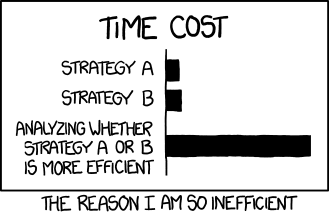
\includegraphics{img/xkcd_1445.png}
\end{center}
\end{frame}
\begin{frame}[plain]
\begin{center}
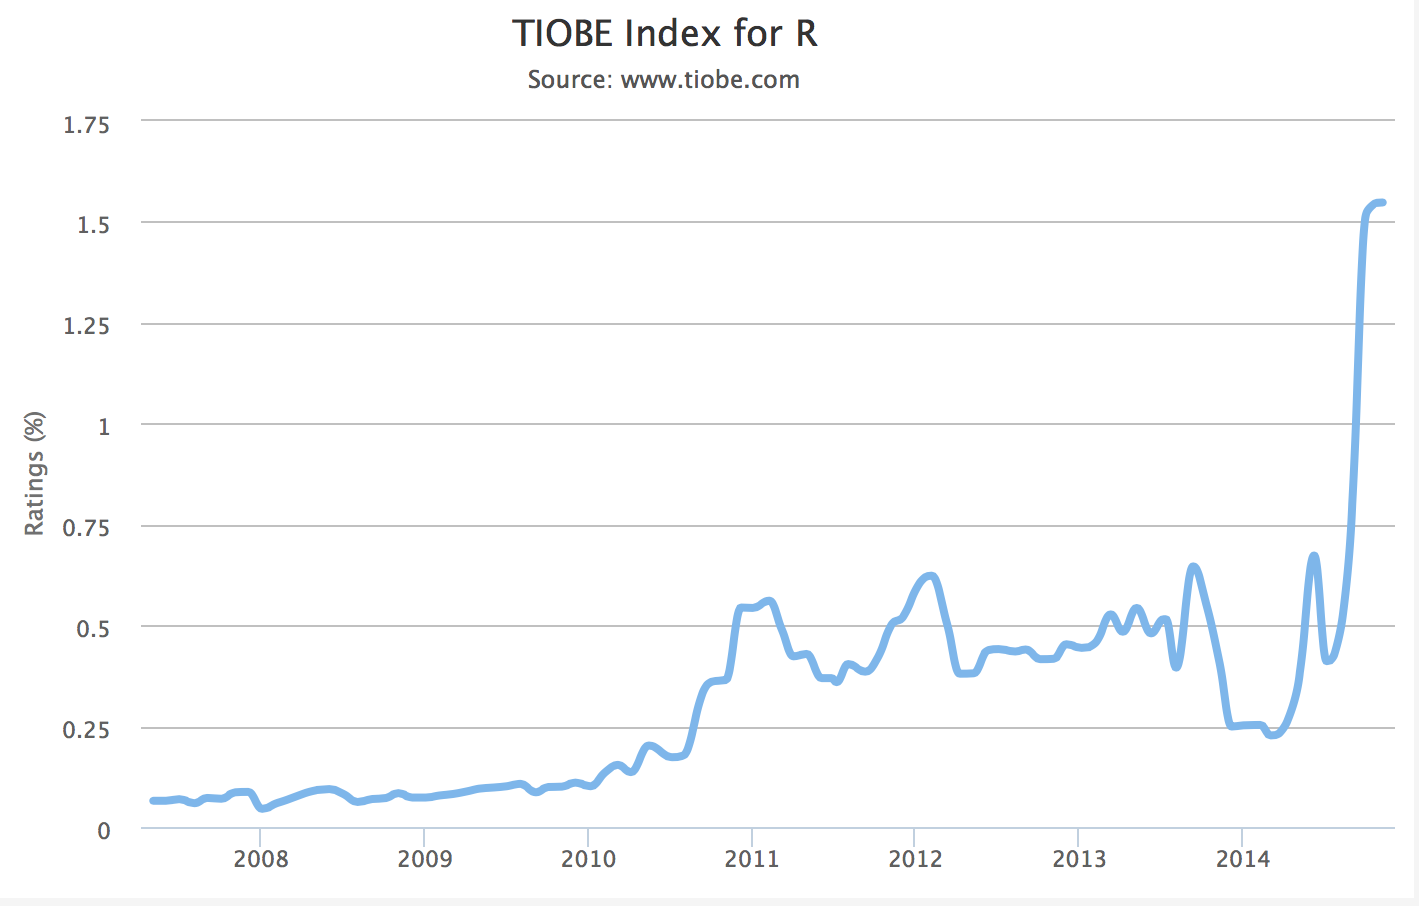
\includegraphics[width=\textwidth]{img/tiobe_r.png}
\end{center}
\end{frame}
\endgroup
\begin{frame}
\frametitle{R...}
\begin{itemize}[<+->]
\item has an \emph{enormous number of packages} for statistical modelling, machine learning, visualization, and importing and manipulating data
\item is designed to \emph{interface} with high-performance computing
languages such as Fortran and C++.
\item can also integrate \emph{web visualizations} from JavaScript libraries such as D3.js,
Leaflet, Google Charts.
\end{itemize}
\end{frame}
\begin{frame}
\frametitle{Bottlenecks}
\begin{itemize}[<+->]
\item The biggest bottleneck in data analysis is cognitive.
\item You need tools (domain specific languages) to help you define the problem and express solutions programmatically.
\end{itemize}
\end{frame}
\begingroup
\begin{frame}[plain]
\vspace{1.5cm}
\begin{center}
\Large\texttt{2. fundamentals}
\end{center}
\end{frame}
\begin{frame}[fragile, plain]
\begin{changemargin}{2.5em}
\begin{lstlisting}
2 + 2
2 * pi
7 + runif(1)
3^4

sqrt(4^4)
log(10)
log(100, base=10)

23 %% 2 # 23 mod 2
23 %/% 2 # floor(23/2)
5e9 * 1e3 # 5000000000 * 1000
\end{lstlisting}
\end{changemargin}
\end{frame}
\begin{frame}[fragile, plain]
\begin{changemargin}{2.5em}
\begin{lstlisting}
val <- 3
val
## [1] 3
print(val)
## [1] 3

val = 1:6
val
## [1] 1 2 3 4 5 6
\end{lstlisting}
\end{changemargin}
\end{frame}
\begin{frame}
\frametitle{R objects}
\begin{itemize}
\item \emph{Vector}: vector of some type (all entries are same type)
\end{itemize}
\end{frame}
\begin{frame}[fragile, plain]
\begin{changemargin}{2.5em}
\begin{lstlisting}
# numeric
nums <- c(1.1, 3, -5.7)
devs <- rnorm(2)
devs
## [1] 1.8469193  0.4091781

# integer
ints <- c(1L, 5L, -3L)
ints
## [1] 1 5 -3
\end{lstlisting}
\end{changemargin}
\end{frame}
% should note single and double string are the same
\begin{frame}[fragile, plain]
\begin{changemargin}{-1.0em}
\begin{lstlisting}
# character
chars <- c('arthur', "marvin's",
           "marvin\"s")
chars
## [1] "arthur" "marvin's" "marvin\"s"

# logical
bools <- c(TRUE, FALSE, TRUE)
bools
## [1] TRUE FALSE TRUE
\end{lstlisting}
\end{changemargin}
\end{frame}
\begin{frame}[fragile, plain]
\begin{changemargin}{-1.0em}
\begin{lstlisting}
vals <- seq(2, 12, by=2)
vals
## [1] 2  4  6  8 10 12
vals[3]
## [1] 6
vals[3:5]
## [1] 6  8 10
vals[c(1, 3, 6)]
## [1] 2  6 12
vals[-c(1, 3, 6)]
## [1] 4  8 10
vals[c(rep(TRUE, 3), rep(FALSE, 4))]
## [1] 2  4  6
\end{lstlisting}
\end{changemargin}
\end{frame}
\begin{frame}[fragile, plain]
\begin{changemargin}{-1.0em}
\begin{lstlisting}
set.seed(42)
vals <- rnorm(3)
vals
## [1]  1.3709584 -0.5646982  0.3631284

vals[1:2] <- 0
vals
## [1] 0.0000000 0.0000000 0.3631284

vals[vals != 0] <- 5
vals
## [1] 0 0 5
\end{lstlisting}
\end{changemargin}
\end{frame}
\begin{frame}[fragile, plain]
\begin{changemargin}{2.5em}
\begin{lstlisting}
vec1 <- 1:3
vec2 <- 3:5
vec1 + vec2
## [1] 4 6 8
vec1 * vec2
## [1] 3 8 15
vec1 >= vec2
## [1] FALSE FALSE FALSE
vec1 <= 3
## [1] TRUE TRUE TRUE
\end{lstlisting}
\end{changemargin}
\end{frame}
\begin{frame}[fragile]
\frametitle{R objects}
\begin{itemize}
\item \emph{Vector}: vector of some type (all entries are same type)
\item \emph{Matrix}: matrix of some type (all entries are same type)
\begin{lstlisting}
mat <- matrix(1:9, nrow = 3)
##      [,1] [,2] [,3]
## [1,]    1    4    7
## [2,]    2    5    8
## [3,]    3    6    9
dim(mat)
class(mat)
t(mat) %*% mat
\end{lstlisting}
\end{itemize}
\end{frame}
\begin{frame}[fragile]
\frametitle{R objects}
\begin{itemize}
\item \emph{Vector}: vector of some type (all entries are same type)
\item \emph{Matrix}: matrix of some type (all entries are same type)
\item \emph{Data frame}: collection of columns (each column can be a different type)
\begin{lstlisting}
dat <- data.frame(ints=1:3,
  chars=c("hello", "world", "foo"))
dat
##   ints chars
## 1    1 hello
## 2    2 world
## 3    3   foo
\end{lstlisting}
\end{itemize}
\end{frame}
\begin{frame}[fragile]
\frametitle{R objects}
\begin{itemize}
\item \emph{Vector}: vector of some type (all entries are same type)
\item \emph{Matrix}: matrix of some type (all entries are same type)
\item \emph{Data frame}: collection of columns (each column can be a different type)
\item \emph{List}: collection of objects
\begin{lstlisting}
list(stuff = 3,
     mat = matrix(1:4, nrow = 2),
     moreStuff = "china",
     list(5, "bear"))
\end{lstlisting}
\end{itemize}
\end{frame}
\begin{frame}[fragile, plain]
\vspace{1.5cm}
\begin{center}
\begin{tabular}{c}
\begin{lstlisting}
help(lm)
?lm
\end{lstlisting}
\end{tabular}
\end{center}
\end{frame}
\begin{frame}[plain]
\vspace{1.5cm}
\begin{center}
\Large\texttt{3. demo}
\end{center}
\end{frame}
\begin{frame}[plain]
\vspace{1.5cm}
\begin{center}
\Large\texttt{4. closer}
\end{center}
\end{frame}
\begin{frame}
\frametitle{Resources}
Guides
\begin{itemize}
\item Text: Hadley Wickham's "\href{http://adv-r.had.co.nz}{Advanced R}"
\item Videos: \href{https://www.youtube.com/watch?v=Bf6XQpyxLq0&list=UUGwuewhdHD2q0BvuB2oWMRw}{2013 R
bootcamp} at UC Berkeley
\item Interactive: \href{https://www.datacamp.com}{DataCamp}
\end{itemize}
\vspace{0.5cm}
Community \& Help
\begin{itemize}
\item \href{http://www.r-project.org/mail.html}{mailing lists}
\item \href{https://twitter.com/hashtag/rstats}{\#rstats}
\item \href{http://www.r-project.org/conferences.html}{useR!}
\item Stack Overflow, Google, Github, ...
\end{itemize}
\vspace{0.5cm}
\end{frame}
\begin{frame}
\frametitle{Resources}
Guides
\begin{itemize}
\item Text: Hadley Wickham's "\href{http://adv-r.had.co.nz}{Advanced R}"
\item Videos: \href{https://www.youtube.com/watch?v=Bf6XQpyxLq0&list=UUGwuewhdHD2q0BvuB2oWMRw}{2013 R
bootcamp} at UC Berkeley
\item Interactive: \href{https://www.datacamp.com}{DataCamp}
\end{itemize}
\vspace{0.5cm}
Help/Community
\begin{itemize}
\item \href{http://www.r-project.org/mail.html}{mailing lists}
\item \href{https://twitter.com/hashtag/rstats}{\#rstats}
\item \href{http://www.r-project.org/conferences.html}{useR!}
\item Stack Overflow, Google, Github, ...
\end{itemize}
\begin{tikzpicture}[remember picture,overlay]
  \node [xshift=0.25cm, yshift=0.25cm, anchor=south west] at (current page.south west) {
    @dustinvtran \tinybullet\
    dustinvtran.com \tinybullet\
    dtran@g.harvard.edu
  };
  \node [xshift=-1.75cm,yshift=1.75cm] at (current page.south east)
    {
\includegraphics[width=2cm,height=2cm]{img/r_logo_flat.png}};
\end{tikzpicture}
\end{frame}
\begin{frame}
\begin{tikzpicture}[remember picture,overlay]
  \node [xshift=0.25cm, yshift=0.25cm, anchor=south west] at (current page.south west) {
    @dustinvtran \tinybullet\
    dustinvtran.com \tinybullet\
    dtran@g.harvard.edu
  };
  \node [xshift=-1.75cm,yshift=1.75cm] at (current page.south east)
    {
\includegraphics[width=2cm,height=2cm]{img/r_logo_flat.png}};
\end{tikzpicture}
\end{frame}
%##############################################################################
% Frames
%##############################################################################
\end{document}
